\chapter{Experiments}
\label{chapter:experiments} 


% \section{Experimental Evaluation Overview}\label{sec:exp}
In this section, we rigorously evaluate our place recognition pipeline to assess its performance in dense forest environments. Our evaluation includes four distinct test sites featuring varying forest compositions: Evo (Finland) characterized by coniferous trees; Stein-Am-Rhein (Switzerland) Wytham Woods (UK) and Forest of Dean (UK) containing both broad-leaf and coniferous tree species. We evaluate all three operational modes of our system: Online SLAM, Offline Multi-Mission SLAM, and Relocalization.
% We can remove the summary of experiments to save space if needed
The experiments conducted are as follows:
\begin{enumerate}[label=\Roman*.]
  \item Evaluation of four different place recognition models at the descriptor-level, tested across multiple forest environments with different LiDAR setups. (\secref{sec:exp_desc_analysis}) 
  \item Performance assessment during both online and offline SLAM operations within dense forest settings. (\secref{sec:exp_online_slam} \& \secref{sec:offline_multi_mission}). \mfallon{somewhere here you need to say you tested only Logg3dNet for some experiments}
  \item Analysis of successful loop closures, based on baseline distance and orientation differences. (\secref{sec:exp_online_slam})
  \item Demonstration of the relocalization application in a previously mapped forest environment, showcasing its utility in an inspection task performed by a quadruped robot. (\secref{sec:exp_relocalization})
\end{enumerate}


% \mfallon{you dont need to cite these papers if you have already introduced them previously}
% \haedam{Okay,edited. Nived: Can you check these 4 key claims?}

% First experiment: descriptors
\section{Place Recognition Descriptors}
\label{sec:exp_desc_analysis} 
In this experiment, we evaluated the descriptors of four different place recognition models (Logg3dNet, EgoNN, ScanContext, STD) focusing on their ability to accurately capture loop-candidates in forest environments. Logg3dNet and EgoNN models are learning-based methods and were pre-trained on the Wild-Places dataset. 
\subsection{Datasets and setups}
We used two different LiDAR sensors mounted on a backpack: Hesai XT32 and Hesai QT64. The XT32 is a long-range, narrow field of view, 32-beams LiDAR, and QT64 is a short-range, wide field of view LiDAR. Note that Wild-Place\cite{knights2023icra} dataset was collected using a inclined VLP-16 LiDAR mounted on spinning motor. This enabled capturing the canopy of the forest, which is difficult for our backpack LiDAR setup. The specifications of the LiDAR sensors used in the experiments are summarized in \tabref{tab:lidar_specs}.
\begin{table}[ht]
  \centering
  \caption{LiDAR Specifications for Mapping}
  \label{tab:lidar_specs}
  \begin{tabular}{|>{\centering\arraybackslash}p{2cm}|>{\centering\arraybackslash}l|c|c|c|}
    \hline
    \multicolumn{1}{|c|}{\textbf{Location}} & \multicolumn{1}{c|}{\textbf{LiDAR}} & \multicolumn{1}{c|}{\textbf{Field of View (\textdegree)}} & \multicolumn{1}{c|}{\textbf{Range (m)}} & \multicolumn{1}{c|}{\textbf{Tree Density}} \\
    \hline
    Wild-Place & VLP-16 & 30 (inclined) & 50 & Low-Medium \\
    \hline
    Evo &  XT32 & 30 & 50 & Medium \\
    \hline
    Stein am Rhein &  XT32 & 30 & 50 & Low \\
    \hline
    Wytham Woods &  QT64 & 100 & 30 & High \\
    \hline
    Forest of Deans & QT64 & 100 & 30 & Low \\
    \hline
  \end{tabular}
\end{table}

\subsection{Precision-Recall Curves}
Precision-recall curves (See \figref{fig:pr_curves}) show how accurately (precision) and frequently (recall) each  model detects correct loop candidates within a reasonable distance threshold (here set to 10\,m) at various descriptor thresholds $\tau_{s}$ in four different forests. Among positive candidates   (whose descriptor distance < $\tau_{s}$ ), we classify them into true positive(\emph{TP}) and false positive(\emph{FP}) depending on whether the candidate is actually located within the loop-closure distance threshold, 10 meter. 
Similarly, among negative candidates, we classify them into true negative(\emph{TN}) and false negative(\emph{FN}) depending on their true location. Thus:
\[ Precision = \frac{TP}{TP + FP} \]
\[ Recall = \frac{TP}{TP + FN} \]

From the precision-recall curves (\figref{fig:pr_curves}), it is evident that Logg3dNet consistently outperforms the other models across the four different forests. Particularly, on the Evo and Stein am Rhein datasets, where a longer range with narrow field of view Hesai XT32 LiDAR was employed, Logg3dNet showed the best performance both in terms of precision and recall, without experiencing any sudden drops in precision.
In contrast, ScanContext demonstrates a significant decrease in precision, attributed to a limited vertical field of view of LiDAR sensor. In more challenging scenarios such as Wytham Woods characterized by complex terrains featuring hills and valleys with dense tree clutter captured with a wide field of view QT64 LiDAR, handcrafted models show a notable decline in performance. However, Logg3dNet remains robust, successfully retrieving a substantial portion of correct loop-candidates, achieving a 70\% precision at a 50\% recall rate. 

% \mfallon{I get to this bit and there is just a hole in the work because nothing about Logg3dNet's algorithm is ever discussed. There is no tuning or ablation. It just presented `as is'.}

To further analyze the distinctiveness of each descriptor, we measured the descriptor distances between all query and database descriptors. This is shown in \figref{fig:heatmap_evo12} as a heatmap, which provides a visual representation of the discriminative potential of each descriptor. Consistent with the precision-recall curves, Logg3dNet descriptors exhibited higher similarity with the ground truth heatmap as observed in the highlighted areas, indicating a high true-positive rate and low false-positive rate, respectively. This implies that Logg3dNet descriptors can effectively detect corresponding loop-candidates during revisits, whereas EgoNN and ScanContext tend to be less discriminative, often returning numerous false-positive candidates. Based on this evidence, we chose Logg3dNet as main the place recognition method for the rest of the experiments.

\begin{figure}[t]
  \centering
  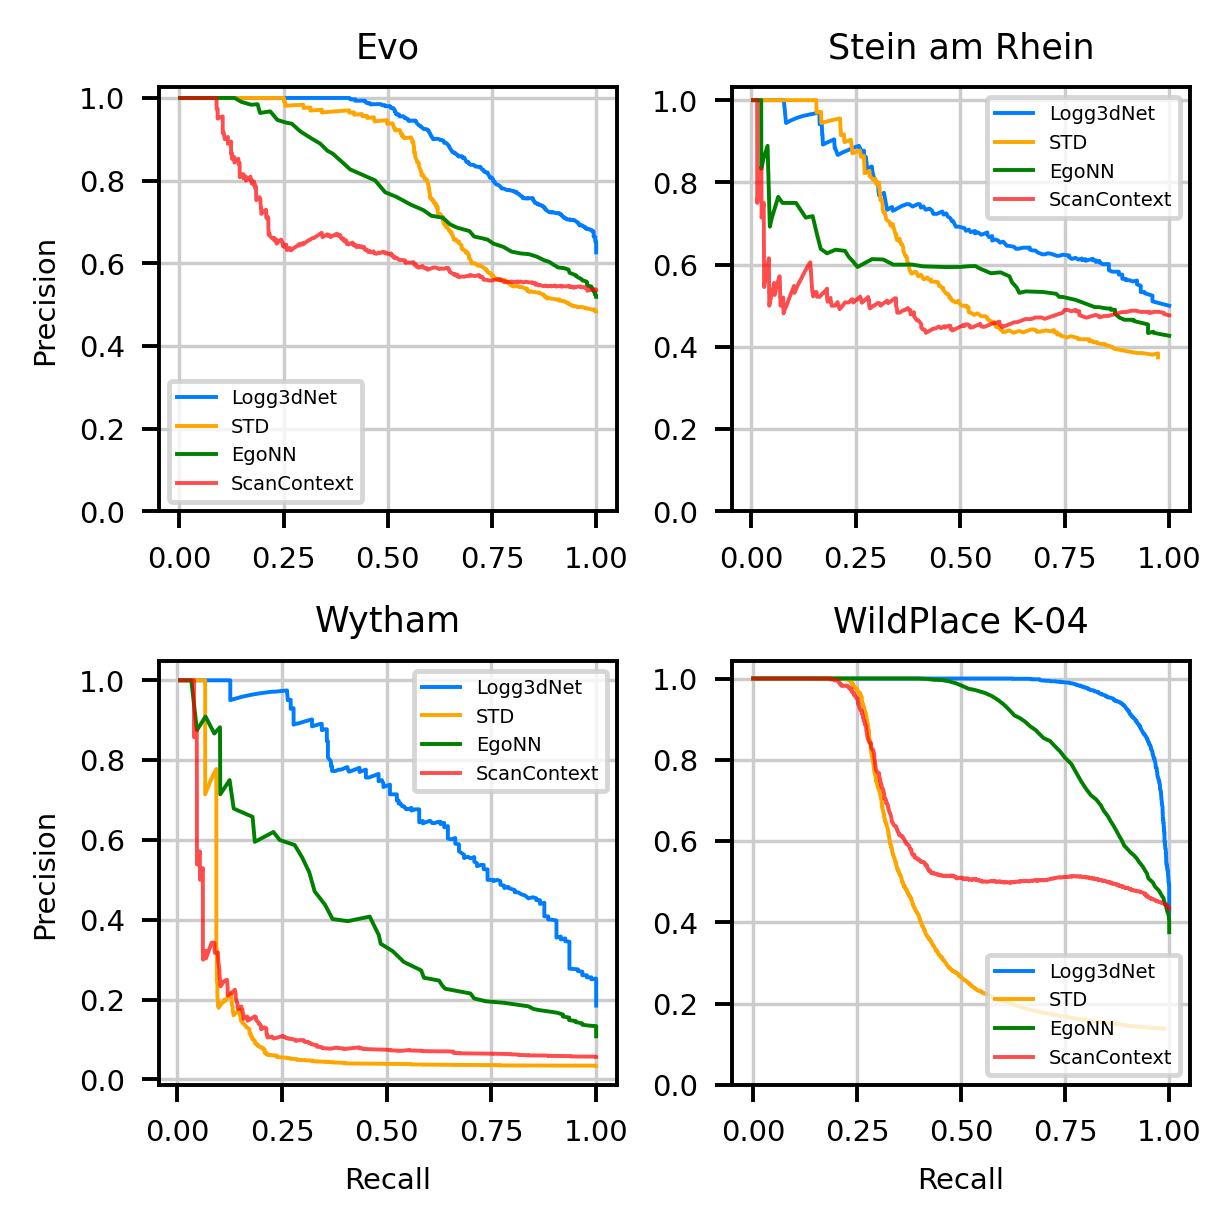
\includegraphics[width=0.99\linewidth]{pics/exp_1.1_pr_curves}
  \caption{Precision-recall curves on four different forest datasets. Evo (Finland, May), Stein am Rhein (Switzerland, Oct), Wytham woods (UK, Feb), Wild-Places \cite{knights2023icra} (Australia).
  Evo and Stein am Rhein datasets were collected by Hesai XT32, and Wytham woods dataset was collected by Hesai QT64. Datasets were collected by backpack-LiDAR within dense forests. Only top-1 candidate within 10\,m of the ground truth position is regarded as a true positive candidate.}
  \label{fig:pr_curves}
\end{figure}


\begin{figure}[t]
  \centering
  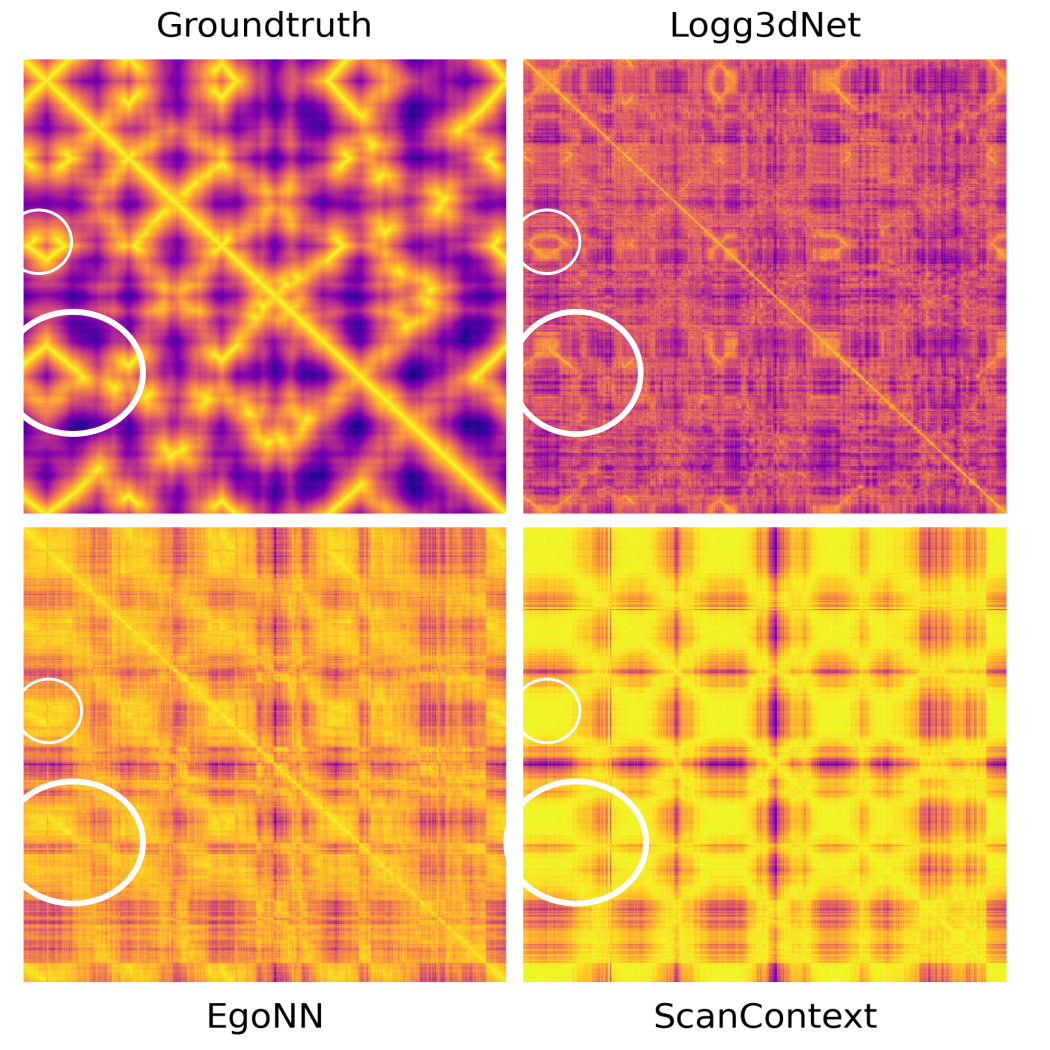
\includegraphics[width=0.99\linewidth]{pics/exp_1.2_heatmap_evo12_plasma_edit}
  \caption{Heatmaps depicting descriptor distances for the Evo dataset. Yellow hues denote a high descriptor similarity between scans, whereas purple indicates the low similarity. Patterns more closely resembling the ground-truth (top-left) indicate better descriptor performance. Logg3dNet descriptors shows the most similar patterns, whereas ScanContext descriptors are least discriminative among these models. We use $\tau_{s}$ that corresponds to the $F_1$-max score in evaluation.}
  \label{fig:heatmap_evo12}
\end{figure}



%%% Second experiment: Online SLAM
\section{Online Place Recognition}
\label{sec:exp_online_slam}
In this experiment, we investigate the online place recognition capability of our system, wherein loop closures from the place recognition module are integrated into the SLAM system. The database $D$, is incrementally built as the sensor moves through the environment. When matching, we exclude the most recent 30 seconds of data to prevent loop closures with immediately recent measurements.
\subsection{Online SLAM}
% Interpret results exp_2_1
\figref{fig:exp_2_1_online_place_recognition} presents an illustrative example of online SLAM performance on the Evo dataset, depicting the sets of loop candidates after each verification step. Initially, many loop closure candidates are proposed (shown in blue) under a descriptor matching threshold $\tau_{s}$ of $F_1$-max score. Loop closures beyond a conservative estimate of \SI{20}{\meter} are rejected using the odometry information. After this, a subset of loop closure candidates are identified using RANSAC matching (highlighted in orange), and finally, a refined set of loop closures that pass the consistency and ICP steps are integrated into the SLAM framework. Final loop closures (shown in red) are one of ICP verified loop candidates by checking pose graph density to avoid over-constraining the pose graph.

\subsection{Loop Closure Statistics}
% Present results in exp2_2
Next, we conducted a comprehensive analysis of loop closure statistics based on distance and viewpoint angles, shown \figref{fig:exp_2_2_loop_closure_histograms}. Our findings show that the system can successfully identify loop closure pairs across considerable baseline distances (\SIrange{10}{20}{\meter}). We observed that despite the large baseline, a significant portion of initial candidates can be registered using RANSAC-based matching, indicating that the correspondences are accurate. However, the proportion of candidates verified by ICP decreases as the distance between scans increases. Specifically, when scans are \SI{10}{\meter} apart, $\sim$\SI{60}{\percent} of RANSAC-registered candidates are successfully verified by ICP, and when \SI{15}{\meter} apart, only $\sim$\SI{40}{\percent} remains verified. This decrease is due to the diminishing overlap ratio between corresponding scans with increasing distance, making convergence of ICP challenging.

Similarly, in terms of viewpoint orientation difference, we observed that a large proportion of the loop candidates up to \SI{90}{\degree} difference are verified both at the RANSAC-registration and ICP-based checks. However, we observed a degradation of performance over \SI{90}{\degree}, which can be attributed to the occlusions in the scans present at large orientation differences. Nonetheless, despite this degradation, the number of final loop closures integrated into the SLAM system proved to be sufficient for correcting the drift.   

% \mfallon{this is worrying and not explained. It's pretty problematic. We should discuss -THIS IS IMPORTANT. There should be no justification for this but we had this problem with Georgi Tinchev's work also. Furthermore, why doesnt it work with the angle is 180d and also 0d. That's quite bad.}
%\haedam{From Initial candidates to Ransac registration there is significant drop across 90-180 ( we can't say it is viewpoint invarient) , but from RANSAC-ICP the proportion is constant. How to explicitly say this ?}

%%% Make this separate figure 
\begin{figure}[t]
  \centering
  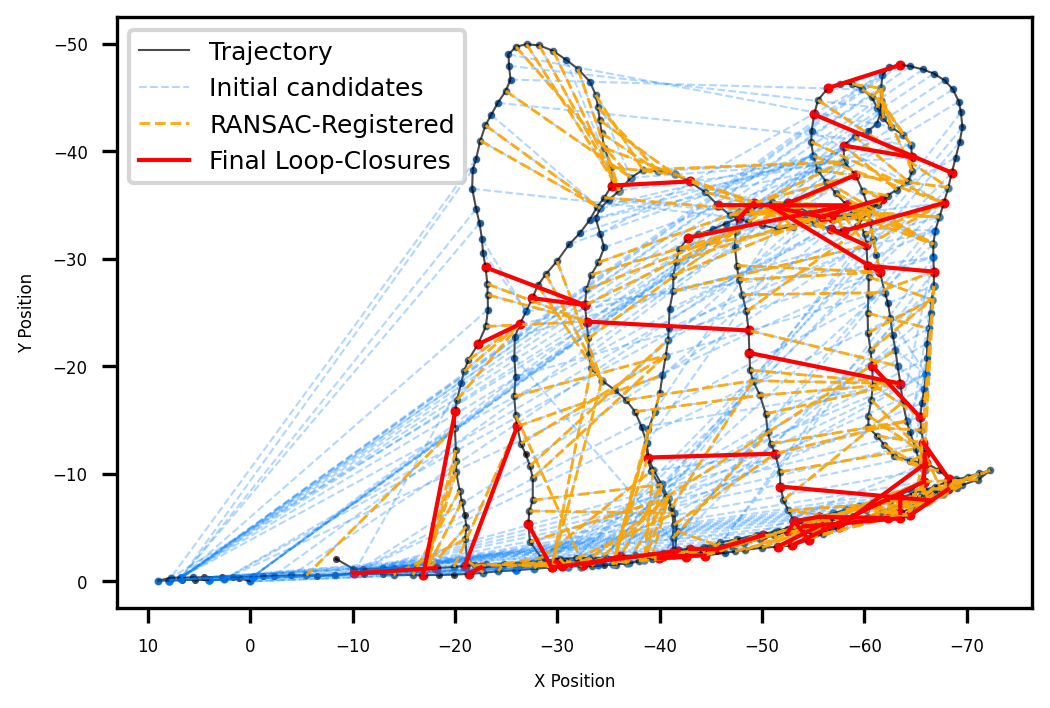
\includegraphics[width=0.99\columnwidth]{pics/exp_2_1_online_place_recognition}
  \caption{Online place recognition on a sequence of the Evo dataset. The sequence covers about 25 minutes of walk with the backpack mapping system (Hesai-XT32). Bold red lines show the loop closures integrated into the SLAM system, successfully identified up to distance of \SI{17}{\meter} within dense forest areas.}
  \label{fig:exp_2_1_online_place_recognition}
\end{figure}

\begin{figure}[t]
  \centering
  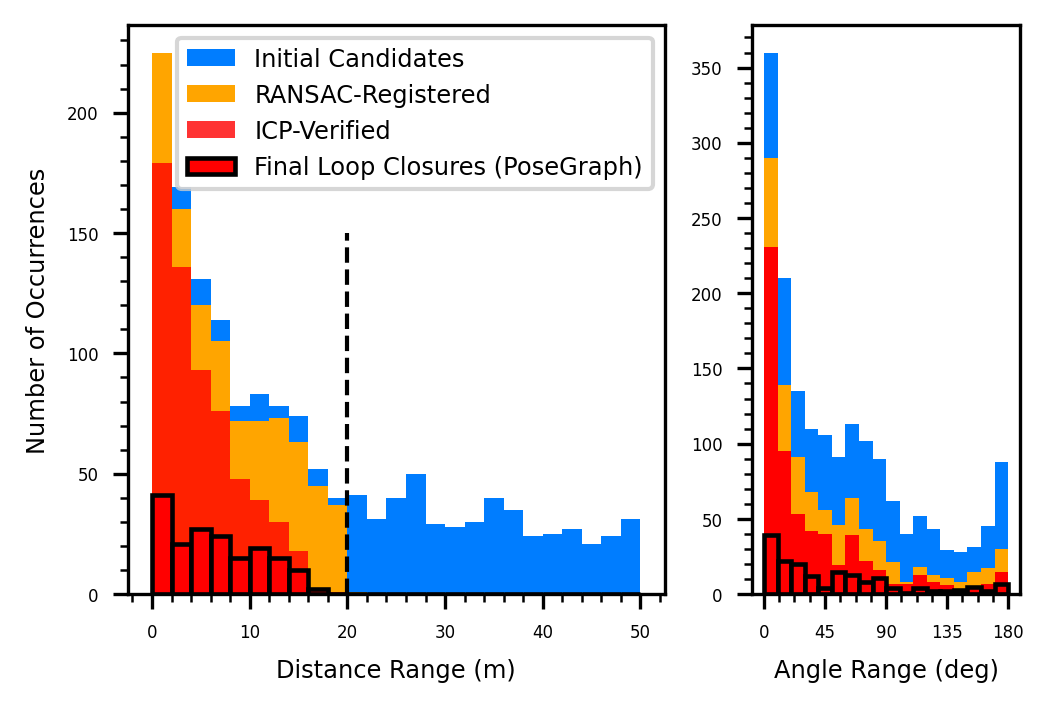
\includegraphics[width=0.99\columnwidth]{pics/exp_2_2_loop_closure_histograms}
  \caption{Loop closures distribution by distance and angle at various stages of the pipeline on Evo dataset.
   Initial candidates based on descriptor distance are shown in blue. Candidates beyond \SI{20}{\meter} are rejected using odometry information. Candidates within \SI{20}{\meter} undergo RANSAC pre-registration with additional verification steps of SGV\cite{vidanapathirana2023ral} and pairwise checks (Yellow). Then these candidates are refined using ICP fine-registration (Red), and final loop closures in the pose graph after checking constraints density in pose graph (red with black outlined).}
  \label{fig:exp_2_2_loop_closure_histograms}
\end{figure}



% Third experiment: Offline Multi-Mission SLAM
%%% 

\begin{figure*}[t]
  \centering
  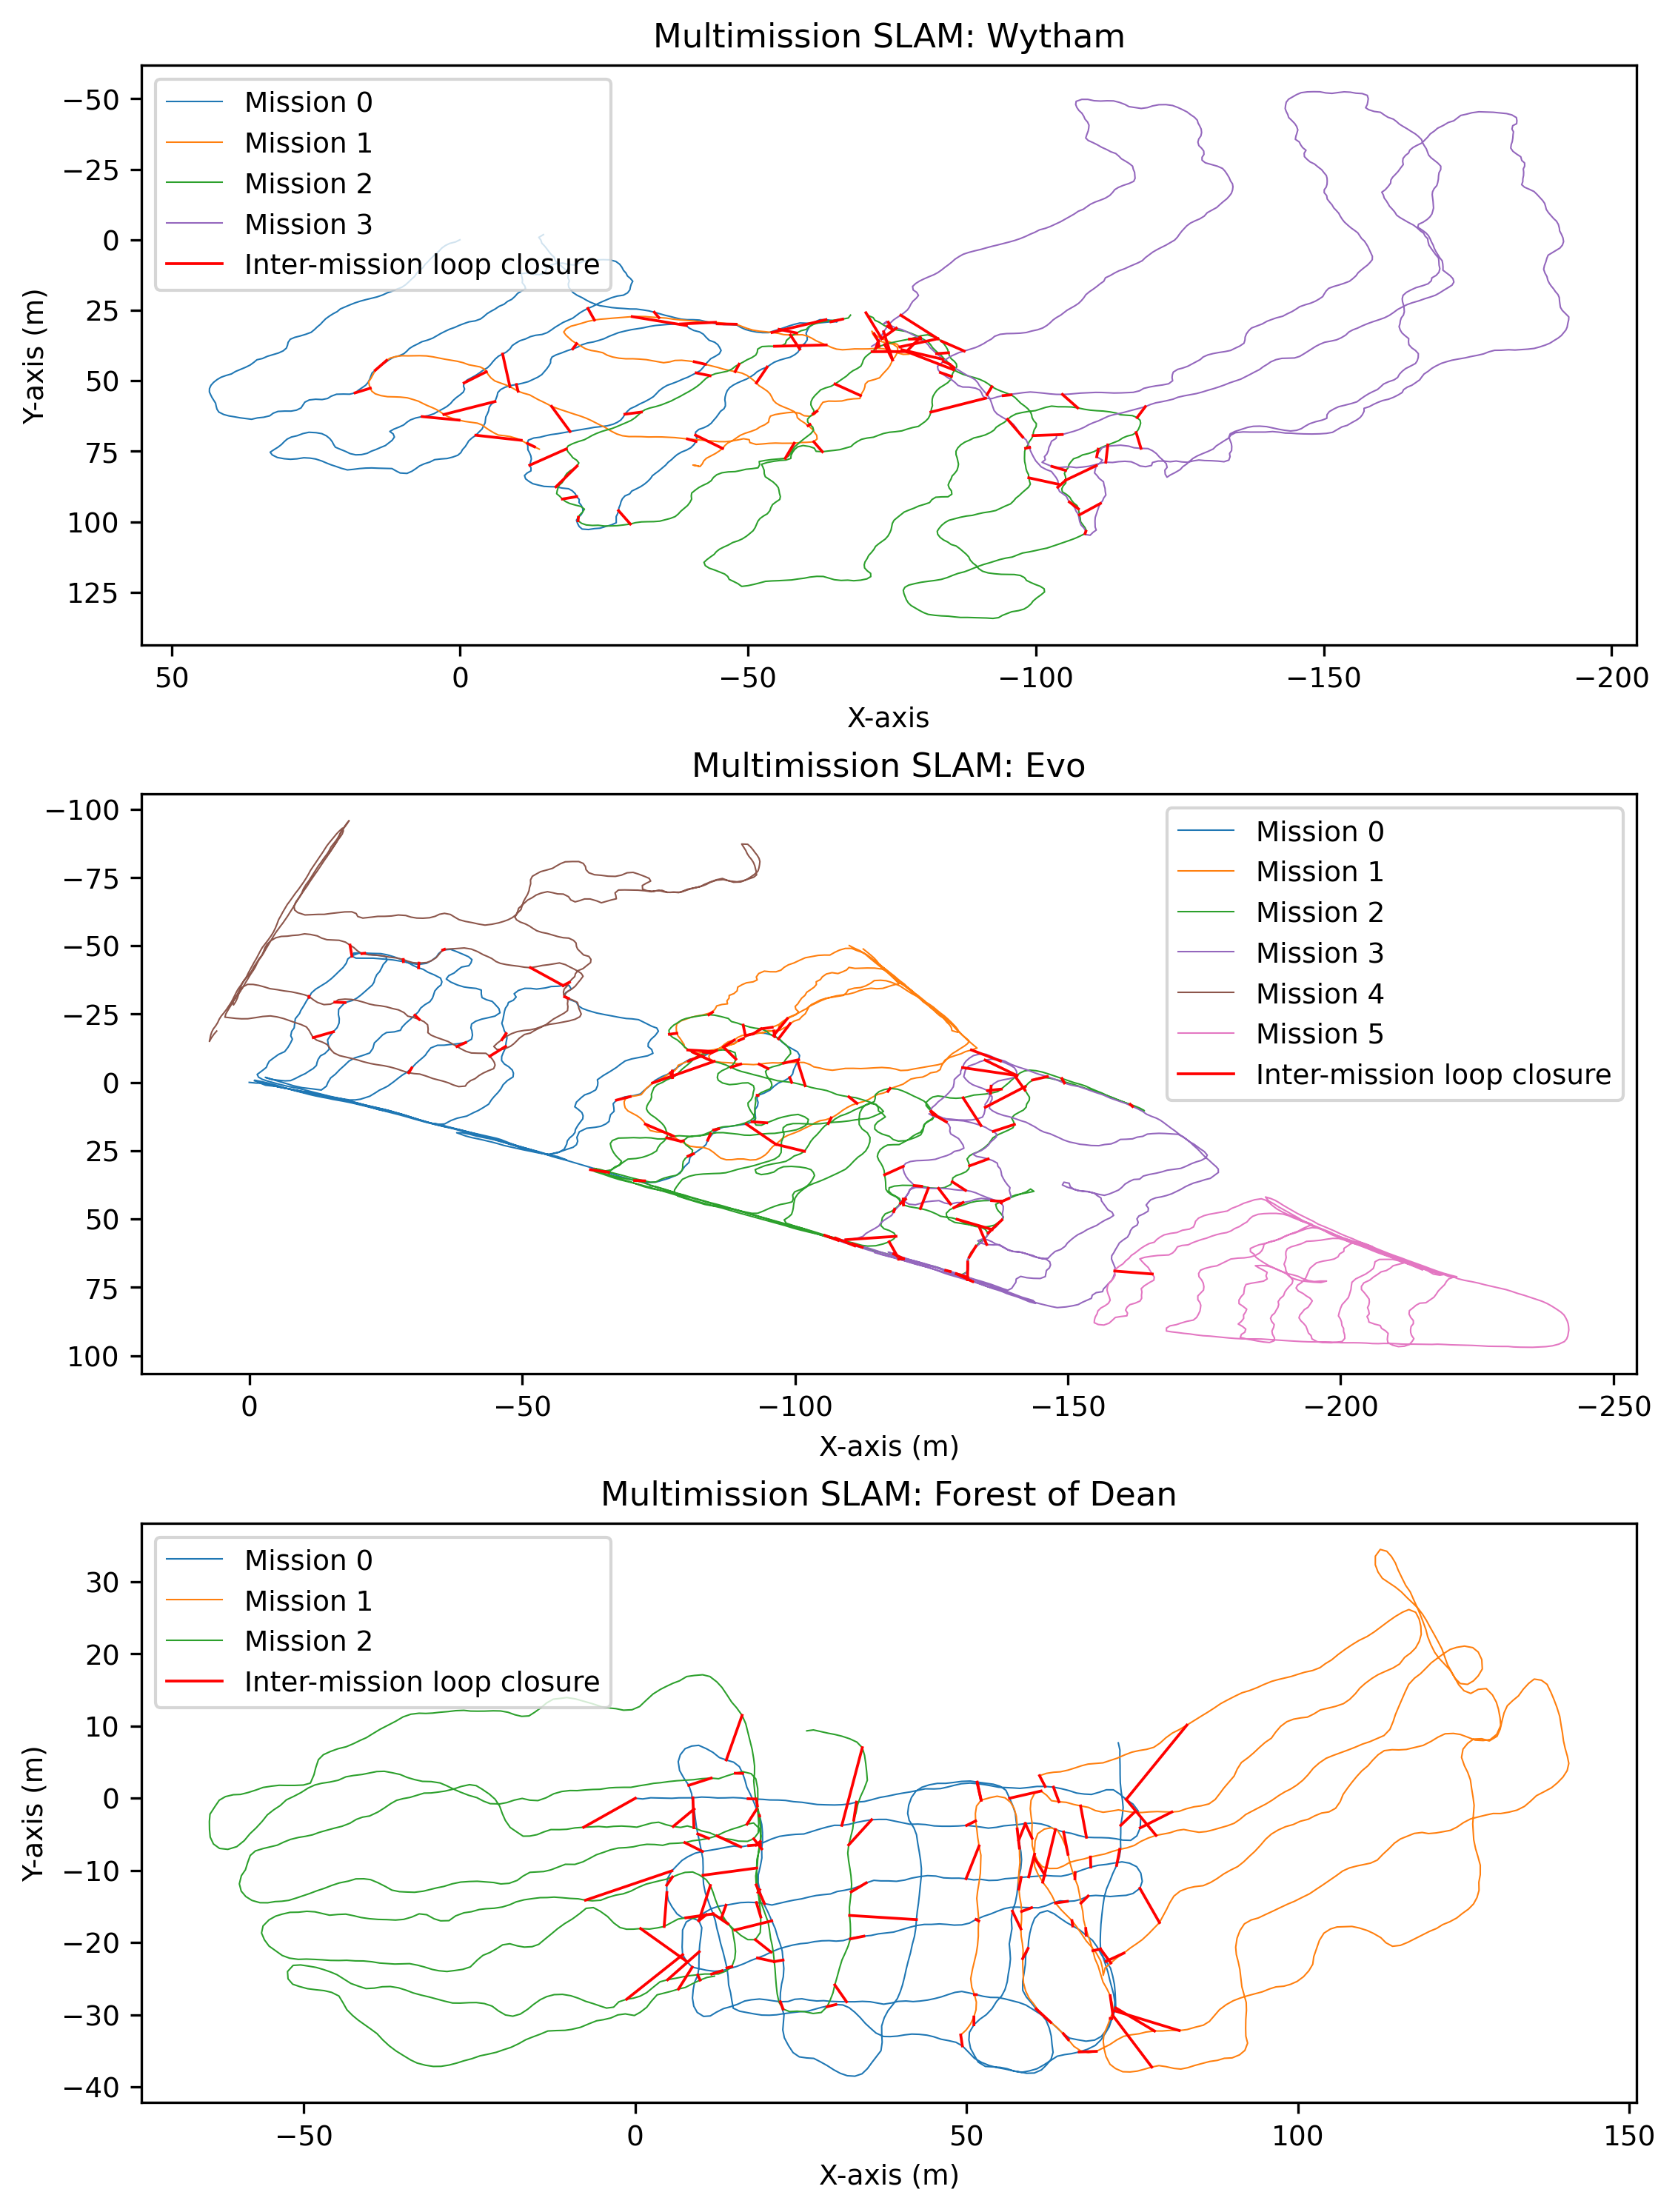
\includegraphics[width=0.99\columnwidth]{pics/exp_3_1_multimission_slam_big}
  \caption{Offline multi-mission SLAM. Left: Wytham - a densely wooded area with uneven terrain, including hills. Center: Evo - featuring a LiDAR setup on an incline, with loop closures occurring primarily when viewpoints are closely aligned. Right: Forest of Dean - flatter terrain compared to Wytham, with a sparser plantation, allowing for loop closures to be captured at greater distances. 
  %\mfallon{please replace yellow - very difficult to see. High importance}
  %\mfallon{blue and purple are difficult to distinguish. Low importance}
}
  \label{fig:exp_multi_mission}
\end{figure*}
\mfallon{I'm interested in the last comment about greater distances. How much?}

\section{Offline Multi-Mission SLAM} 
\label{sec:offline_multi_mis  sion}
In this experiment, we showcased the ability of our approach to obtain loop closures between different mapping missions and to merge those missions into a common map. In this task, we employed tighter descriptor thresholds ($\tau_{s}$) compared to the online SLAM task, in order to reduce the number of false positive loop candidates.
Figure \ref{fig:exp_multi_mission} presents the results of merging different sequences within three different datasets: Wytham Woods, Evo, and the Forest of Dean. Each individual mission covers approximately one hectare, with merged map areas ranging from three to five hectares.
% \mfallon{these details about sensors should have been mentioned before hand. can you introduce the two sensors in the start of the experiments and refer to them ad the Wide FOV and Narrow FOV lidar afterwards.}
We observed that there were more frequent \emph{intermission} loop closures in the Forest of Dean compared to Wytham in overlapping areas. This can be attributed to the higher tree density, foliage, and vegetation present in Wytham, making the descriptors less distinctive.     

Further, we tested the robustness of our system on the Evo multi-mission dataset, where the XT32 LiDAR was placed at a \SI{45}{\degree} inclination aimed at capturing the forest canopy. Despite the asymmetry in point clouds introduced by this inclination change, which primarily captured points in the forward direction, our approach successfully identified loop closures and achieved multi-mission map merging.

Overall, our experiments showed potential for efficient large-scale mapping, as we did not require to start at the open access roads nor following exactly the same paths to achieve loop closures between inter-missions. We also built the map incrementally, one section at a time, hence overlapping areas could only be guaranteed for subsequent missions.

% \tabref{tab:exp_offline_distance_table} provides summary statistics of the distribution of loop closures at different distance ranges. Our multi-stage verification pipeline effectively filters out unreliable loop candidates, with approximately 90\% of successful candidates found within 10\,m of each other. Notably, experiments conducted in Wytham Woods and the Forest of Dean highlight that our system can identify loop closures within the forests, eliminating the need to precisely retrace previously mapped areas to achieve loop closures. This underscores the versatility and robustness of our approach in real-world forest mapping scenarios.

%MF: I removed these comments. I dont think they were adding
%, and facilitates loop-closures with much smaller overlapping areas between inter-missions
%Also, most of them occurred at the start and end of each missions. 



%\mfallon{The name is `Forest of Dean'. It is not Deans or Dean. It is always `Forest of Dean'}


\begin{table}[htbp]
  \centering
  \small
  \begin{tabular}{p{2cm}cccc}
      \toprule
      \multicolumn{1}{l}{loop closures} & \multicolumn{3}{c}{Dataset} \\
      \multicolumn{1}{l}{distance range (m)} & Wytham & Evo & Forest of Dean \\
      \midrule
      0-5\,m &41 / 53\%  &83 / 78\%  &73 / 78\% \\
      \midrule
      5-10\,m &29 / 37\%  &19 / 18\% &15 / 16\%\\
      \midrule
      10-15\,m &8 / 10\%  &4 / 4\%   &6 / 6\% \\
      \midrule
      Total  & 78 / 100\%  & 106 / 100\%  & 94 / 100\% \\
      \bottomrule
  \end{tabular}
  \caption{Offline Multi-mission map merging results corresponding to \figref{fig:exp_multi_mission}: Number and percentage of final inter-mission loop closures detected by distance between matched poses.
  %Setting rigorous thresholds on number of descriptors, SGV, pairwise consistency check and ICP registration allows robust loop-closure pairs to be found, with any loop-candidates more than 15m away rejected.
  }  
  \label{tab:exp_offline_distance_table}
\end{table}
\mfallon{I don't know what this table is supposed to be saying}


\begin{figure}[t]
  \centering
  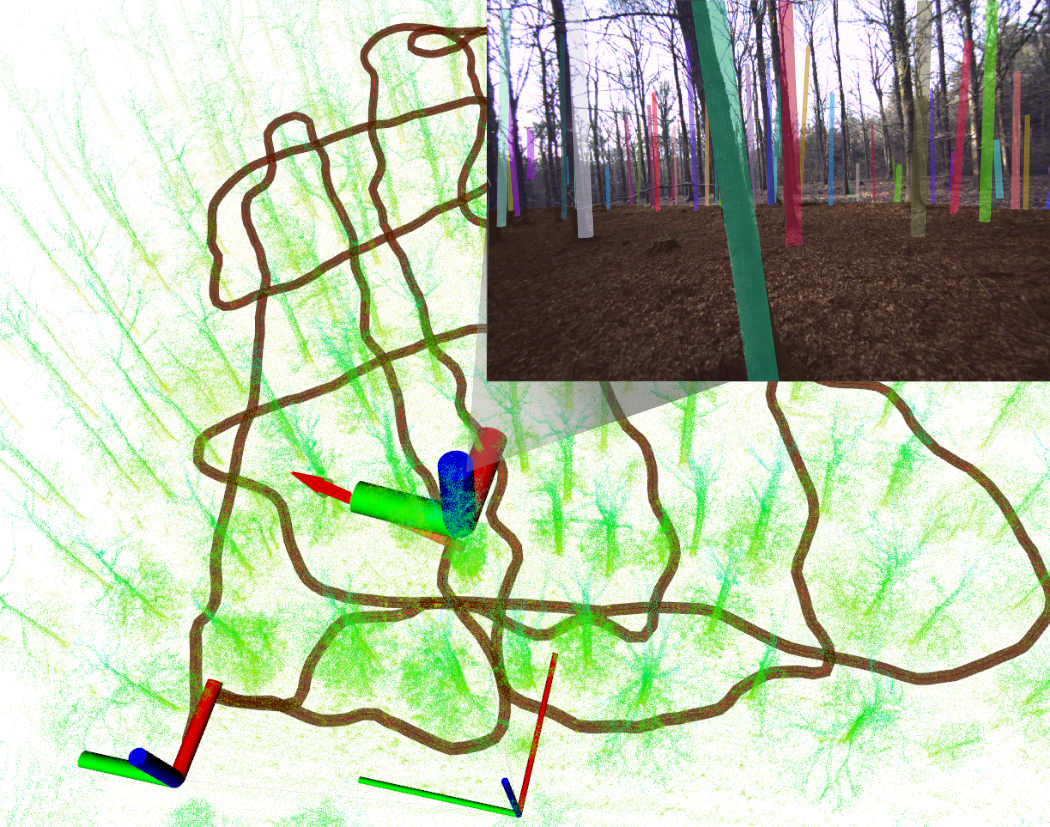
\includegraphics[width=0.99\linewidth]{pics/relocalization_demo.png}
  \caption{Demonstration of relocalization capability. LiDAR (illustrated by large marker) is relocalized in a prior map. We render a virtual view of the forest digital map synchronized with images from our camera (right). Red arrow shows a successful localization at that pose.
  }
  \label{fig:relocalization}
\end{figure}

% Fourth experiment: Relocalization 
\section{Relocalization} 
\label{sec:exp_relocalization}
% What is this experiment about?
This experiment showcases a relocalization demonstration in a dense forest using our approach. In this scenario, our system demonstrates the ability to continuously track the position within a prior SLAM map once an initial loop closure is established.
% What are some particular characteristic?
%Unlike multi-mission, since prior map poses are fixed as ground truth,  we no longer jointly optimize poses.
%Instead, we found that precision of 6DOF localization itself affects pairwise consistency of loop-closures.
%Therefore, we limit the pairwise consistency threshold at few centimeter level. This enables continuous relocalization only within centimeter level of error, while reducing recall. 
Figure \ref{fig:relocalization} presents an illustrative example of this demonstration, where the quadruped robot shown in \mfallon{Fig 1} is localized with respect to a prior SLAM map generated using a backpack LiDAR system. This capability enables the real-time rendering of a virtual forest map overlaid with associated data, such as Diameter at Breast Height (DBH) and species information, onto the camera images. Such feedback is highly beneficial for tasks such as taking forest inventories by foresters or enabling autonomous harvesting.

%\mfallon{Dont use the word CAD. CAD is relevant to mechanical designs - not trees. Use `virtual' }

%\mfallon{can you swap the images to that you talk about prior map (left) and then virtual rendering (right). Because English is read from left to right}

%%%%%%%%%%%%%%%%%%%%%%%%
\section{Study of ICP inlier-based check}
\label{sec:exp_icp_ablation}

Our final experiment investigates the ICP inlier-based check on loop closure integration within the final pose graph optimization process. This analysis is crucial for ensuring that incorrect loop closures are not introduced into the optimized pose graph.
\figref{fig:ablation_icp_inliers} illustrates the corrections (on top of the initial transformation prior) as estimated by the ICP registration at various distances. Additionally, the figure color-codes the points based on the number of inlier points obtained during the registration process, with blue indicating a large number of inliers and red indicating a smaller number.
Our observation suggests that loop closures occurring beyond 10\,m, which propose a substantial transformation correction often have fewer inlier ICP points and are thus less reliable.
Based on this analysis, we establish an inlier threshold to ensure that corrections are limited to ICP corrections of less than 1 meter (shown in dotted red line). This threshold further reduces the number of incorrect loop closures from being integrated into the pose graph.

\mfallon{I'd like to discuss this also, but it reads fine}

% What is the interpretation of the figure?
% Alongside \figref{fig:exp_2_2_loop_closure_histograms}, further analysis has been done how robust the loop-candidates are. 
% \figref{fig:ablation_icp_inliers} shows that under 10m distance, ICP inliers are high as over 4k points, and correction error is below 1m. However, the distribution of loop-candidates start to diverge significantly after 10m: correction error no longer bounds to 1m and the number of inliers are much less than 4k points. 
% Setting a low ICP inlier threshold will provide far distance loop-closures, but there is a chance of getting False Positives.

\begin{figure}[t]
  \centering
  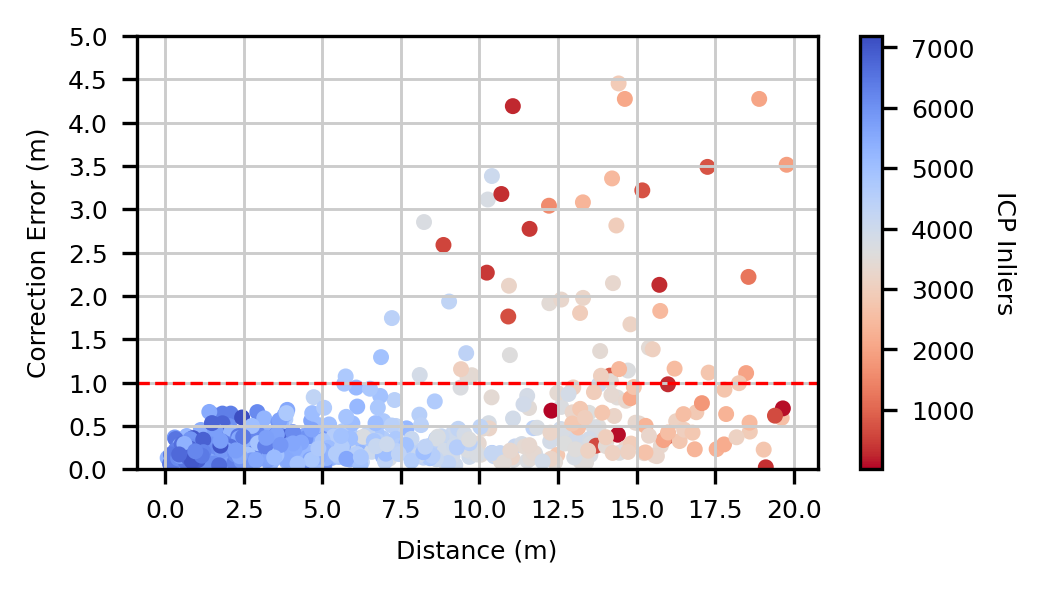
\includegraphics[width=0.99\linewidth]{pics/exp_4_ablation_icp_inliers_4cm}
  \caption{Analysis of final ICP registration check. X-axis shows the distribution of loop-candidates by distance after ICP.
  Y-axis shows ICP correction error w.r.t. the coarse-registration from RANSAC. Color indicates the number of ICP inliers,  30 iterations and RMSE= 0.01m, where clouds are cropped 50 by 50m, then downsampled to 20k points. \haedam{reduce size}}
  \label{fig:ablation_icp_inliers}
\end{figure}
\mfallon{this caption is too brief for a reader to parse what is meant by all the variables.}
